% Created 2020-05-21 Thu 11:40
% Intended LaTeX compiler: pdflatex
\documentclass[presentation]{beamer}
\usepackage[utf8]{inputenc}
\usepackage[T1]{fontenc}
\usepackage{graphicx}
\usepackage{grffile}
\usepackage{longtable}
\usepackage{wrapfig}
\usepackage{rotating}
\usepackage[normalem]{ulem}
\usepackage{amsmath}
\usepackage{textcomp}
\usepackage{amssymb}
\usepackage{capt-of}
\usepackage{hyperref}
\RequirePackage{fancyvrb}
\DefineVerbatimEnvironment{verbatim}{Verbatim}{fontsize=\scriptsize}
\usetheme{metropolis}
\usecolortheme{}
\usefonttheme{}
\useinnertheme{}
\useoutertheme{}
\author{Petru Rebeja, Marius Apetrii}
\date{14 Mai 2020}
\title{Tehnici Avansate de Programare}
\subtitle{Database design \& Introducere în DevOps}
\institute[UAIC]{Facultatea de Matematică\\Universitatea Alexandru Ioan Cuza, Iași}
\hypersetup{
 pdfauthor={Petru Rebeja, Marius Apetrii},
 pdftitle={Tehnici Avansate de Programare},
 pdfkeywords={},
 pdfsubject={},
 pdfcreator={Emacs 26.3 (Org mode 9.3.6)},
 pdflang={Romanian}}
\begin{document}

\maketitle
\section{Introducere}
\label{sec:org4507d23}
\begin{frame}[label={sec:orgfa5e7a6},fragile]{Recapitulare}
 \pause
\begin{itemize}
\item \texttt{TPL} simplifică integrarea execuţiei paralele şi asincrone în aplicaţie lăsând în grija sistemului detaliile de nivel inferior a.î. programatorul să se poată concentra asupra logicii aplicaţiei.
\end{itemize}
\pause
\begin{itemize}
\item \texttt{Middleware} sunt componentele care fac parte din linia de procesare a interogărilor şi răspunsurilor la interogări. Ex: middleware pentru autentificare şi autorizare.
\end{itemize}
\pause
\begin{itemize}
\item \texttt{Autentificare} --- procesul de preluare a datelor care atestă identitatea unui utilizator şi verificarea acestora; implementat de \texttt{ASP.NET Core Identity}.
\end{itemize}
\pause
\begin{itemize}
\item \texttt{Autorizare} --- procesul de verificare a drepturilor de acces a  unui utilizator în vederea accesării unei anumite resurse; se face cu ajutorul \texttt{AuthorizeAttribute}.
\end{itemize}
\end{frame}
\begin{frame}[label={sec:org648bfb8}]{Agenda}
\begin{itemize}
\item Proiectarea bazelor de date
\begin{itemize}
\item Relaţii
\item Forme normale
\item Proiectare
\end{itemize}
\item DevOps
\begin{itemize}
\item Continuous Integration
\item Continuous Delivery
\item Continuous Deployment
\end{itemize}
\item Demonstraţii
\end{itemize}
\end{frame}
\section{Proiectarea bazelor de date}
\label{sec:org44a424f}
\begin{frame}[label={sec:org4826ff4},fragile]{Primary/Foreign Key}
 \begin{itemize}
\item O cheie primară (\texttt{Primary Key}) este o mulţime de coloane ale unui tabel a căror valori identifică în mod unic o înregistrare\footnote{\url{http://www.differencebetween.net/technology/difference-between-primary-key-and-unique-key/}}.
\item O cheie străină (\texttt{Foreign Key}) este o mulţime de coloane ale unui tabel care fac referinţă la o cheie primară\footnote{\url{https://www.w3schools.com/sql/sql\_foreignkey.asp}}.
\end{itemize}
\end{frame}
\begin{frame}[label={sec:org240b2f0},fragile]{Relaţie}
 Adăugarea unei chei străine crează o \texttt{relaţie} între cele două tabele unde:
\begin{itemize}
\item Tabelul \texttt{copil} este cel care conţine cheia străină,
\item Tabelul \texttt{părinte} este cel care conţine cheia primară referenţiată de tabelul copil.
\end{itemize}
\end{frame}
\begin{frame}[label={sec:orgda7bc8e}]{Exemplu: 1*N}
\begin{center}
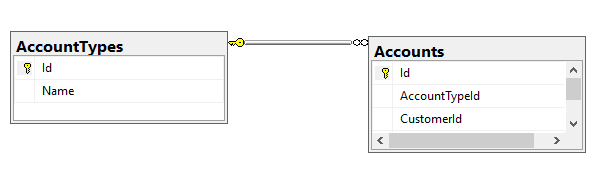
\includegraphics[width=\textwidth]{img/one-to-many.png}
\end{center}
\end{frame}
\begin{frame}[label={sec:org3a9b201}]{Exemplu\footnote{\url{https://smehrozalam.wordpress.com/2010/06/29/entity-framework-queries-involving-many-to-many-relationship-tables/}}: N*M}
\begin{center}
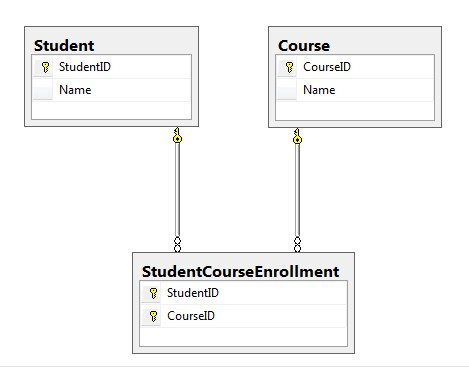
\includegraphics[width=.8\textwidth]{img/many-to-many.png}
\end{center}
\end{frame}
\begin{frame}[label={sec:org8245fac}]{Normalizare}
\begin{block}{Normalizarea bazei de date}
\vskip 0.1in
Procesul de structurare a unei baze de date relaţionale pentru a reduce redundanţa datelor şi a îmbunătăţi integritatea acestora\footnote{\url{https://en.wikipedia.org/wiki/Database\_normalization}}.
\end{block}
\end{frame}
\begin{frame}[label={sec:org32624b9}]{Objective normalizare}
\begin{itemize}
\item Modelarea conceptelor din lumea reală şi a relaţiilor dintre acestea.
\item Extensibilitate sporită: adăugarea obiectelor noi se face cu intervenţie minimă.
\end{itemize}
\end{frame}
\begin{frame}[label={sec:org710ca13},fragile]{Forme normale}
 \begin{itemize}
\item Normalizarea se face prin aducerea schemei la o \texttt{formă normală}.
\item O \texttt{formă normală} este o proprietate a structurii bazei de date.
\item Există mai multe forme normale (\texttt{FN1}---\texttt{FN6} etc.).
\item O bază de date este normalizată dacă respectă cel puţin \texttt{FN3}.
\end{itemize}
\end{frame}
\begin{frame}[label={sec:orga3ce708},fragile]{Forma Normală 1}
 \begin{block}{FN1}
\vskip 0.1in
O relaţie este în \texttt{Forma Normală 1} dacă în fiecare coloană a unui tabel avem doar valori atomice.
\end{block}
\end{frame}
\begin{frame}[label={sec:org15c5547},fragile]{Forma Normală 1}
 Normalizarea la \texttt{FN1} se face prin:
\begin{enumerate}
\item Eliminarea grupurilor care se repetă.
\item Crearea unui table pentru fiecare colecţie de date cu coeziune mare.
\item Adăugarea unei chei primare.
\end{enumerate}
\end{frame}
\begin{frame}[label={sec:org1192849},fragile]{Forma Normală 2}
 \begin{block}{FN2}
\vskip 0.1in
O relaţie este în \texttt{Forma Normală 2} dacă:
\begin{enumerate}
\item Este în \texttt{Forma Normală 1} şi
\item Toate atributele unui tabel depind doar de cheia primară direct sau indirect.
\end{enumerate}
\end{block}
\end{frame}
\begin{frame}[label={sec:orgceb3a30}]{Forma Normală 2}
Tournament winners\footnote{\url{https://en.wikipedia.org/wiki/Third\_normal\_form}}
\begin{center}
\begin{tabular}{lrll}
\uline{Tournament} & \uline{Year} & Winner & Winner's date of birth\\
\hline
Indiana Invitational & 1998 & Al Fredrickson & 21 July 1975\\
Cleveland Open & 1999 & Bob Albertson & 28 September 1968\\
Des Moines Masters & 1999 & Al Fredrickson & 21 July 1975\\
Indiana Invitational & 1999 & Chip Masterson & 14 March 1977\\
\end{tabular}
\end{center}
\end{frame}
\begin{frame}[label={sec:org1fc37d1},fragile]{Forma Normală 3}
 \begin{block}{FN3}
\vskip 0.1in
O relaţie este în \texttt{Forma Normală 3} dacă:
\begin{enumerate}
\item Este în \texttt{Forma Normală 2} şi
\item Fiecare atribut depinde direct de cheia primară.
\end{enumerate}
\end{block}
\end{frame}
\begin{frame}[label={sec:orgc95e252}]{Forma Normală 3\footnote{\url{https://en.wikipedia.org/wiki/Third\_normal\_form}}}
\begin{center}
\begin{tabular}{lrl}
Tournament & Year & Winner\\
\hline
Indiana Invitational & 1998 & Al Fredrickson\\
Cleveland Open & 1999 & Bob Albertson\\
Des Moines Masters & 1999 & Al Fredrickson\\
Indiana Invitational & 1999 & Chip Masterson\\
\end{tabular}
\end{center}
\begin{center}
\begin{tabular}{ll}
Winner & Date of birth\\
\hline
Chip Masterson & 14 March 1977\\
Al Fredrickson & 21 July 1975\\
Bob Albertson & 28 September 1968\\
\end{tabular}
\end{center}
\end{frame}
\section{DevOps}
\label{sec:org632df36}
\begin{frame}[label={sec:orge08479f},fragile]{DevOps}
 \begin{block}{DevOps}
\vskip 0.1in
Un set de practici care combină dezvoltarea software (\texttt{Dev}) şi logistica IT (\texttt{Ops}) a cărui scop este să reducă durata ciclului de dezvoltare software şi să crească frecvenţa de livrare a sistemelor software\footnote{\url{https://en.wikipedia.org/wiki/DevOps}}.
\end{block}
\end{frame}
\begin{frame}[label={sec:orgbec45a7},fragile]{Conductele de livrare}
 \begin{block}{Deployment pipeline}
\vskip 0.1in
Procesul \uline{automat} prin care codul-sursă este preluat din sistemul de gestiune al istoricului şi transformat într-un artefact (\texttt{deliverable}) prin care sistemul software poate fi pus la dispoziţia utilizatorilor.
\end{block}
\end{frame}
\begin{frame}[label={sec:org1ac25f9}]{Conductele de livrare: Motivaţie}
\begin{itemize}
\item Automatizarea procesului elimină riscul de eroare umană
\item Timpii de aşteptare constanţi
\item Creşte încrederea în calitatea produsului
\end{itemize}
\end{frame}
\begin{frame}[label={sec:org0849343}]{Exemplu\footnote{\url{https://www.linux.com/audience/devops/devops-fundamentals-part-4-patterns-and-practices/}}}
\begin{center}
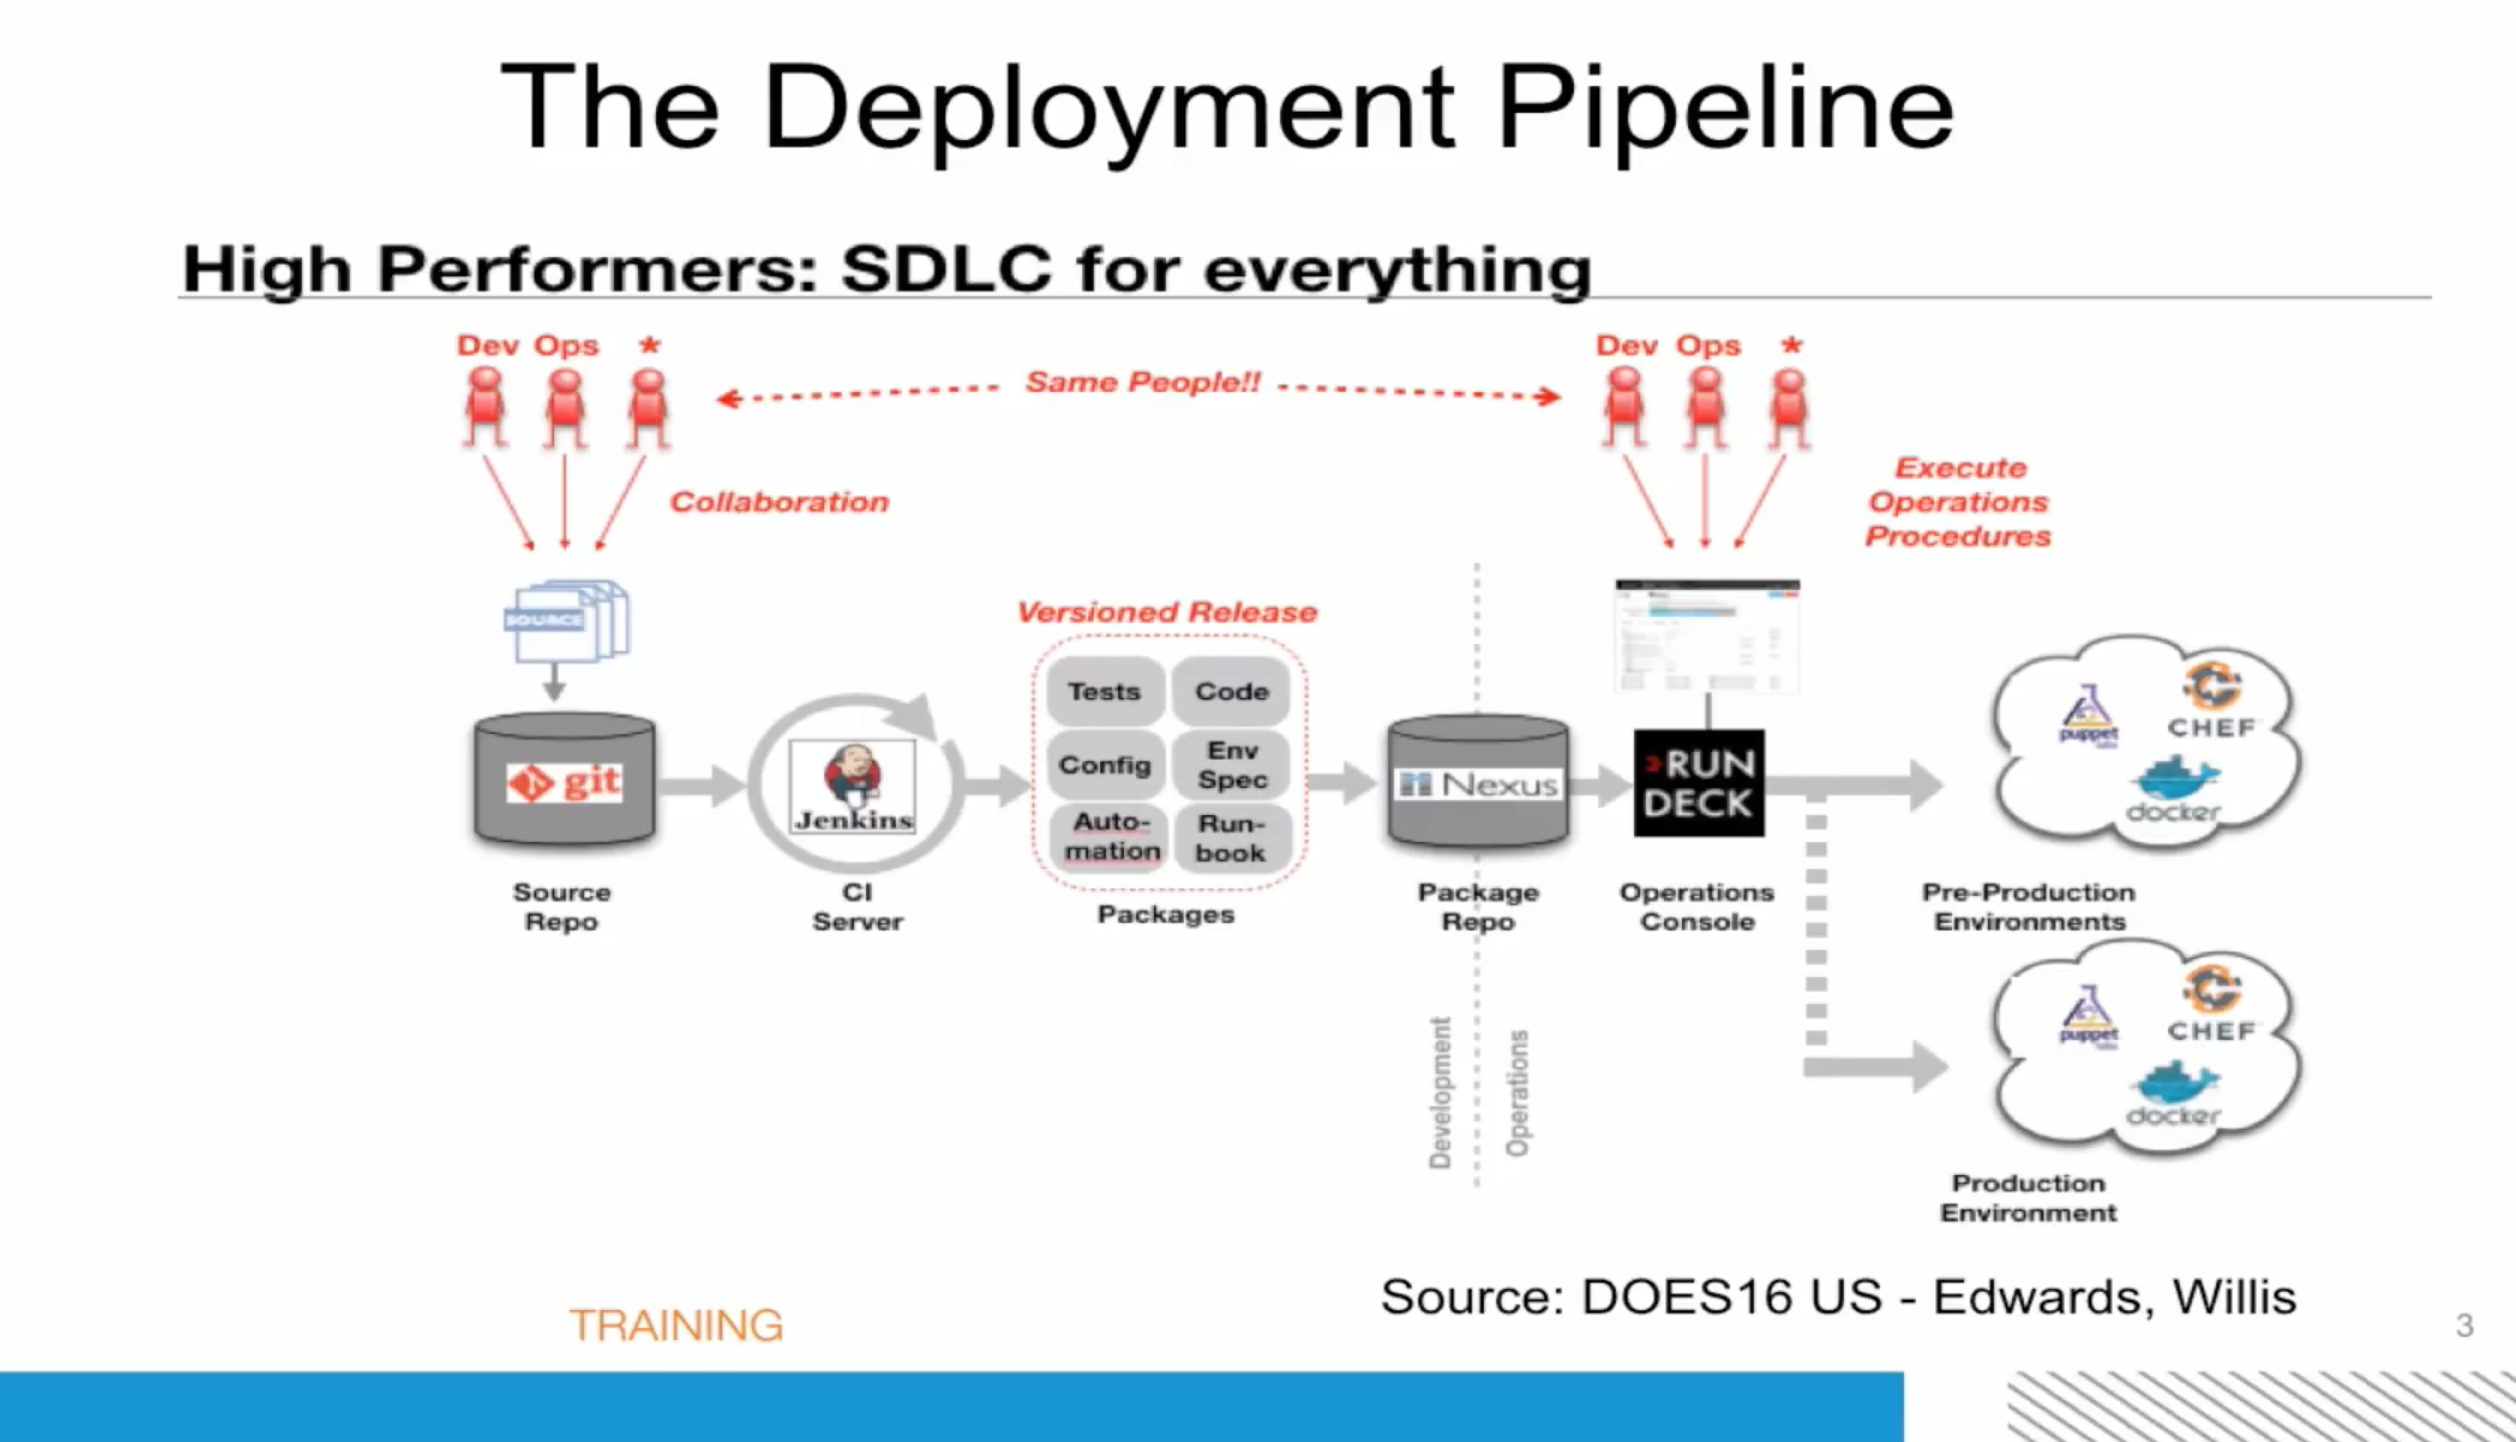
\includegraphics[width=\textwidth]{img/deployment-pipeline.png}
\end{center}
\end{frame}
\begin{frame}[label={sec:org66bcacb}]{Continuous Integration}
\begin{block}{Continuous Integration}
\vskip 0.1in
Practică a dezvoltării software în care modificările aduse de fiecare programator în parte sunt integrate în sistemul de gestine al istoricului şi verificate în mod automat.
\end{block}
\end{frame}
\begin{frame}[label={sec:org4375936}]{Continuous Delivery}
\begin{block}{Continuous Delivery\footnote{\url{https://www.martinfowler.com/bliki/ContinuousDelivery.html}}}
\vskip 0.1in
Practică a dezvoltării software în care aplicaţia poate fi lansată în producţie în orice moment.
\begin{itemize}
\item Necesită intervenţie umană.
\end{itemize}
\end{block}
\end{frame}
\begin{frame}[label={sec:org616ee5f}]{Continuous Deployment}
\begin{block}{Continuous Deployment}
\vskip 0.1in
Practică a dezvoltării software în care orice modificare nouă a aplicaţiei este lansată în mod automat în producţie.
\end{block}
\end{frame}
\section{Demonstraţii}
\label{sec:org0322eb4}
\section{Încheiere}
\label{sec:orgee205eb}
\begin{frame}[label={sec:orgc90892a},fragile]{Recapitulare}
 \pause
\begin{itemize}
\item Elemente esenţiale în proiectarea bazelor de date: \texttt{cheie primară}, \texttt{cheie străină} şi \texttt{relaţie}.
\end{itemize}
\pause
\begin{itemize}
\item \texttt{Normalizare} --- proiectarea/restructurarea bazei de date pentru a o aduce în (cel puţin) \texttt{forma normală 3}.
\end{itemize}
\pause
\begin{itemize}
\item \texttt{Practicile DevOps} pentru creşterea frecvenţei de livrare.
\end{itemize}
\pause
\begin{itemize}
\item \texttt{Conductele de livrare} --- ne ajută să implementăm practici precum:
\begin{itemize}
\item \texttt{Continuous Integration} --- integrarea şi verificarea automată a modificărilor,
\item \texttt{Continous Delivery} --- posibilitatea de a trimite oricând aplicaţia în producţie,
\item \texttt{Continuous Deployment} --- lansarea automată în producţie a modificărilor noi.
\end{itemize}
\end{itemize}
\end{frame}
\begin{frame}[label={sec:org58f89da}]{Vă mulțumesc!}
\begin{center}
Mulțumesc pentru atenție!
\end{center}
\end{frame}
\end{document}